\documentclass[11pt]{article}

\usepackage[margin=1in]{geometry}
\usepackage{listings}
\usepackage{graphicx}
\usepackage{subfigure}
\usepackage{subcaption} % For subfigures
\usepackage{float} % for H option in figures
\usepackage{url}
\usepackage{float}
\usepackage{amsfonts}
\usepackage{hyperref}

\usepackage{biblatex} %Imports biblatex package
\addbibresource{../../../source/bibliography.bib} %Import the bibliography file

\setlength{\parindent}{0pt}

\title{What is a nnU-Net?}
\author{Anton Zhitomirsky}

\begin{document}

\maketitle

This is a sumamry of the contents of the file \cite{nnunet} and example of its implementation (from the github \cite{nnunet-git-paper}).

\section{Summary of \cite{nnunet}}

Similarly to the original U-Net architecture they don't change much, but since they are now dealing with 3D data, they consider a pool of basic U-Net architectures: 2D U-Net (\ref{sec:2d-u-net}), a 3D U-Net (\ref{sec:3d-u-net}) and a U-Net Cascade (\ref{sec:u-net-cascade}).

\subsection{2D U-Net} \label{sec:2d-u-net}

Contrary to belief that using a 2D network in the context of a 3D network may be counter-intuitive, the paper found that 3D segmentation methods deteriorate in performance if the dataset is anisotropic \cite{nnunet} (when the property varies according to direction \cite{anisotropy}).

\subsection{3D U-Net}\label{sec:3d-u-net}

The architecture would typically thrive on contextual information, but we are limited by GPU memory, which allows us to train this architecture only on image patches. This may pose a problem for generating PTV areas because of the large structures, which, in size, may be compared to a Liver which has been cited as `large images such as Liver, may impede training' \cite{nnunet}.

\subsection{U-Net Cascade} \label{sec:u-net-cascade}

While the 2D and 3D U-Nets generate segmentations at full resolution, the cascade first generates low resolution segmentations and subsequently refines them.

This addresses the shortcoming in Section \ref{sec:3d-u-net} because we first train the 3D U-Net on downsampled images (which compresses the amount of contextual information you need) (stage 1) and then upsamples to the original voxel spacing and passed as additional (one hot encoded) input channels to a second 3D U-Net, which is trained on patches at full resolution (stage 2).

\begin{figure}[H]
    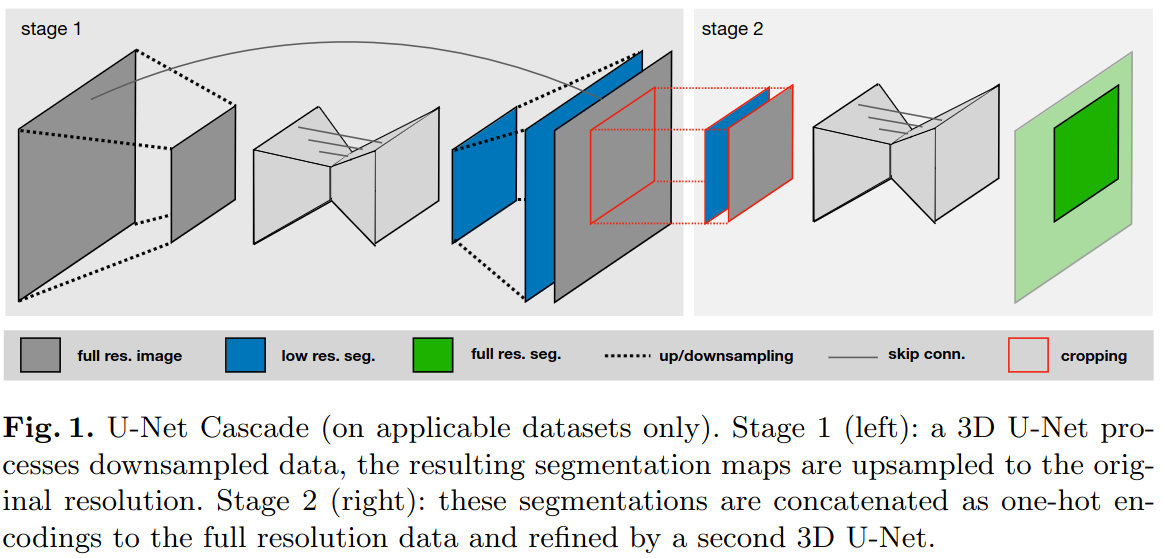
\includegraphics[width=\linewidth]{images/nnunet-diagram.png}
\end{figure}

\section{Summary of \cite{nnunet-git-paper}}

This paper focuses more on the out-of-the-box aspect of training a neural network on a dataset.

We have a three step recipe to follow to allow for no intervention from the user when it comes to defining custom parameters based on the structure the u-net is analysing:

\subsection{Fixed Parameters}

During development of nnU-Net we identified a robust configuration (that is, certain architecture and training properties) that can simply be used all the time. This includes, for example, nnU-Net's loss function, (most of the) data augmentation strategy and learning rate.

\begin{itemize}
    \item Architectural template: closely follows U-Net, uses Leaky ReLU instead of ReLU.
    \item Training schedule: 1000 epochs with 250 mini-batches
    \item Inference: sliding window
\end{itemize}

\subsection{Rule-based Parameters}

Uses the dataset fingerprint to adapt certain segmentation pipeline properties by following hard-coded heuristic rules. For example, the network topology (pooling behavior and depth of the network architecture) are adapted to the patch size; the patch size, network topology and batch size are optimized jointly given some GPU memory constraint.

\begin{itemize}
    \item intensity normalisation
    \item Resampling
    \item target spacing
    \item Adaptation of network topology, patch size and batch size.
    \item Initialization
    \item Architectural topology
    \item Adaptation to GPU memory budget.
    \item Batch size
    \item Configuration of the 3D U-Net cascade.
\end{itemize}

\subsection{Empirical Parameters}

trial-and-error. For example the selection of the best U-net configuration for the given dataset (2D, 3D full resolution, 3D low resolution, 3D cascade) and the optimization of the postprocessing strategy.

\begin{itemize}
    \item Ensembling and selection of U-Net configuration(s)
    \item Post-processing
\end{itemize}

\subsection{Data Fingerprint}

\begin{itemize}
    \item As a first processing step, nnU-Net crops the provided training cases to their non-zero region (improved computational efficiency)
    \item captures fingerprint like: \begin{itemize}
        \item image size (before and after cropping)
        \item image spacing (phyiscal size of voxels)
        \item modalities (x-ray, ultrasound, ct, etc...)
        \item as well as mean and std of all voxels
    \end{itemize}
\end{itemize}

\printbibliography

\end{document}